\documentclass[aspectratio=169, 10pt]{beamer}

\usepackage[utf8]{inputenc}
\usepackage[T5]{fontenc}
\usepackage[vietnamese]{babel}
\usepackage{helvet}
\usepackage{times}
\usepackage{fontawesome5}
\usepackage{booktabs}
\usepackage{colortbl}
\usepackage{xcolor}
\definecolor{rowGray}{gray}{0.95}
\usepackage{colortbl}
\usepackage{booktabs}
\usepackage{multirow}
\usepackage{amsmath, amssymb}
\usepackage{graphicx}
\usepackage{subcaption}
\usepackage{tikz}
\usepackage{pgfplots}
\pgfplotsset{compat=1.18}
\usepackage{tcolorbox}
\usetikzlibrary{positioning, arrows.meta, shapes.geometric, shadows}
\usepackage{pifont}
\tcbuselibrary{skins, raster}
\usetikzlibrary{tikzmark, calc, arrows.meta, positioning}

\definecolor{primaryDark}{RGB}{0, 51, 102}
\definecolor{primaryLight}{RGB}{0, 85, 150}
\definecolor{targetBg}{RGB}{253, 237, 236}
\definecolor{accentTeal}{RGB}{0, 100, 100}
\definecolor{alertRed}{RGB}{220, 50, 50}
\definecolor{textBlack}{RGB}{30, 30, 30}
\definecolor{lightGrayBg}{RGB}{245, 245, 245}

\usetheme{Madrid}
\usecolortheme{default}

% --- Phông chữ báo cáo chuyên nghiệp (Times serif) cho nội dung slide ---
% Trang bìa giữ nguyên phông Helvetica (xem {
\setbeamertemplate{background}{
\begin{tikzpicture}[overlay, remember picture]
    \fill[primaryDark] (current page.south west) rectangle (current page.north east);
    \fill[primaryLight] (current page.south west) -- (current page.south east) -- (current page.north east) -- cycle;
    \fill[primaryDark!80] (current page.west) rectangle ([xshift=0.5\paperwidth]current page.west);
    \fill[accentTeal!70] ([yshift=-0.08\paperheight]current page.south west) rectangle ([xshift=0.42\paperwidth, yshift=0.08\paperheight]current page.south west);
    \fill[accentTeal!50] ([yshift=0.3\paperheight]current page.south west) rectangle ++(0.03\paperwidth, 0.6\paperheight);
\end{tikzpicture}
}
\setbeamertemplate{navigation symbols}{}

\begin{frame}[plain]
    \centering
    
    \vspace{0.5cm}
    
    {\color{white}\fontsize{7}{9}\selectfont\textmd{ĐẠI HỌC TÔN ĐỨC THẮNG}}
    \par{\color{white!70}\fontsize{6}{8}\selectfont\textmd{KHOA CÔNG NGHỆ THÔNG TIN}}
    
    \vspace{0.5cm}
    
    {\color{white}\fontsize{8}{10}\selectfont\textbf{DỰ ÁN CÔNG NGHỆ THÔNG TIN}}
    
    \vspace{0.25cm}
    
    {\color{accentTeal!80}\fontsize{7}{9}\selectfont\textbf{BÁO CÁO TIẾN ĐỘ NGHIÊN CỨU}}
    
    \begin{tikzpicture}
        \draw[accentTeal, line width=0.4mm] (0,0) -- (5,0);
    \end{tikzpicture}
    
    \vspace{0.3cm}
    
    {\color{white}\fontsize{13}{17}\selectfont\textbf{XÂY DỰNG MẠNG CAMPUS NETWORK}}
    \par{\color{white}\fontsize{13}{17}\selectfont\textbf{SỬ DỤNG SDN VÀ SD-WAN}}
    
    \vspace{0.45cm}
    
    \begin{tikzpicture}
        \draw[white!30, line width=0.2mm] (0,0) -- (5,0);
    \end{tikzpicture}
    
    \vspace{0.4cm}
    
    {\color{white}\fontsize{6}{7}\selectfont
    \begin{tabular}{lc}
        \textbf{Giảng viên hướng dẫn:} & {\color{white!80}ThS. Lê Viết Thanh} \\[0.12cm]
        \textbf{Sinh viên thực hiện:} & {\color{white!80}Trần Hữu Nhân -- 52300235} \\[0.05cm]
        & {\color{white!80}Nguyễn Nhật Hào -- 52300198}
    \end{tabular}
    }
    
    \vspace{0.45cm}
    
    {\color{white!50}\fontsize{5}{6}\selectfont\today}
    
\end{frame}
}
).
% Lưu ý: KHÔNG dùng \setbeamerfont{...}{family=ptm} — key `family` (thiếu dấu `*`)
% lưu tên phông như text thô, bị typeset ra chữ "pt" ở góc trang.
\renewcommand{\familydefault}{\rmdefault}

\setbeamercolor{structure}{fg=primaryDark}
\setbeamercolor{palette primary}{bg=primaryDark, fg=white}
\setbeamercolor{palette secondary}{bg=primaryLight, fg=white}
\setbeamercolor{palette tertiary}{bg=accentTeal, fg=white}
\setbeamercolor{frametitle}{bg=primaryDark, fg=white}
\setbeamercolor{title}{bg=primaryDark, fg=white}
\setbeamercolor{block title}{bg=primaryDark, fg=white}
\setbeamercolor{block body}{bg=lightGrayBg, fg=textBlack}
\setbeamercolor{alerted text}{fg=alertRed}

\setbeamertemplate{navigation symbols}{}
\setbeamertemplate{itemize item}{\color{accentTeal}$\blacksquare$}
\setbeamertemplate{itemize subitem}{\color{accentTeal}$\bullet$}
\setbeamertemplate{enumerate item}{\color{primaryDark}\textbf{\insertenumlabel.}}

% --- Tiêu đề hiện đại: thanh bên trái + gạch chân kiểu khối vuông ---
\setbeamercolor{headlineRule}{bg=accentTeal}
\setbeamertemplate{frametitle}{%
  \begin{beamercolorbox}[wd=\paperwidth,ht=0.9cm,dp=0.1cm,leftskip=0.55cm,rightskip=0.55cm]{frametitle}%
    \begin{tikzpicture}[remember picture,overlay]
      \fill[accentTeal]
        ([xshift=0cm,yshift=-0.15cm]current page.north west)
        rectangle ++(0.18cm,-0.75cm);
    \end{tikzpicture}%
    \insertframetitle
  \end{beamercolorbox}%
  \begin{beamercolorbox}[wd=\paperwidth,ht=2.5pt]{headlineRule}%
  \end{beamercolorbox}%
}

% --- Footer hiện đại: gạch viền trên + nền tối, cân trang ---
\setbeamercolor{footline}{bg=primaryDark, fg=white!80}
\setbeamertemplate{footline}{%
  \begin{beamercolorbox}[wd=\paperwidth,ht=1.5pt]{headlineRule}%
  \end{beamercolorbox}%
  \begin{beamercolorbox}[wd=\paperwidth,ht=3.1ex,dp=1.2ex,leftskip=0.55cm,rightskip=0.55cm]{footline}%
    \small\textbf{\insertshorttitle}\hfill\textbf{Trang \insertframenumber/\inserttotalframenumber}
  \end{beamercolorbox}%
}

% --- Block hình chữ nhật, không bo góc (hiện đại, phẳng) ---
\renewenvironment{block}[1]{%
  \begin{tcolorbox}[enhanced, sharp corners=all, arc=0pt,
    colback=lightGrayBg, colframe=accentTeal, boxrule=1pt,
    left=7pt, right=7pt, top=4pt, bottom=4pt,
    before skip=0pt, after skip=0pt,
    title={#1}, fonttitle=\bfseries,
    coltitle=white, colbacktitle=primaryDark,
    boxed title style={sharp corners=all, arc=0pt, boxrule=0pt,
      colback=primaryDark, left=7pt, right=7pt, top=2pt, bottom=2pt},
    leftrule=3pt, rightrule=0.5pt, toprule=0.5pt, bottomrule=0.5pt
  ]}{%
  \end{tcolorbox}%
}

\title[SDN \& SD-WAN Campus]{\texorpdfstring{XÂY DỰNG MẠNG CAMPUS NETWORK\\SỬ DỤNG SDN VÀ SD-WAN}{XÂY DỰNG MẠNG CAMPUS NETWORK SỬ DỤNG SDN VÀ SD-WAN}}
\subtitle{Báo cáo tiến độ nghiên cứu -- Dự án Công nghệ Thông tin}
\author[Trần Hữu Nhân -- Nguyễn Nhật Hào]{Trần Hữu Nhân -- 52300235; Nguyễn Nhật Hào -- 52300198}
\institute[]{Khoa Công nghệ Thông tin -- Đại học Tôn Đức Thắng}
\date{\today}

\begin{document}

% Trang bìa giữ nguyên phông Helvetica
{\fontfamily{phv}\selectfont
{
\setbeamertemplate{background}{
\begin{tikzpicture}[overlay, remember picture]
    \fill[primaryDark] (current page.south west) rectangle (current page.north east);
    \fill[primaryLight] (current page.south west) -- (current page.south east) -- (current page.north east) -- cycle;
    \fill[primaryDark!80] (current page.west) rectangle ([xshift=0.5\paperwidth]current page.west);
    \fill[accentTeal!70] ([yshift=-0.08\paperheight]current page.south west) rectangle ([xshift=0.42\paperwidth, yshift=0.08\paperheight]current page.south west);
    \fill[accentTeal!50] ([yshift=0.3\paperheight]current page.south west) rectangle ++(0.03\paperwidth, 0.6\paperheight);
\end{tikzpicture}
}
\setbeamertemplate{navigation symbols}{}

\begin{frame}[plain]
    \centering
    
    \vspace{0.5cm}
    
    {\color{white}\fontsize{7}{9}\selectfont\textmd{ĐẠI HỌC TÔN ĐỨC THẮNG}}
    \par{\color{white!70}\fontsize{6}{8}\selectfont\textmd{KHOA CÔNG NGHỆ THÔNG TIN}}
    
    \vspace{0.5cm}
    
    {\color{white}\fontsize{8}{10}\selectfont\textbf{DỰ ÁN CÔNG NGHỆ THÔNG TIN}}
    
    \vspace{0.25cm}
    
    {\color{accentTeal!80}\fontsize{7}{9}\selectfont\textbf{BÁO CÁO TIẾN ĐỘ NGHIÊN CỨU}}
    
    \begin{tikzpicture}
        \draw[accentTeal, line width=0.4mm] (0,0) -- (5,0);
    \end{tikzpicture}
    
    \vspace{0.3cm}
    
    {\color{white}\fontsize{13}{17}\selectfont\textbf{XÂY DỰNG MẠNG CAMPUS NETWORK}}
    \par{\color{white}\fontsize{13}{17}\selectfont\textbf{SỬ DỤNG SDN VÀ SD-WAN}}
    
    \vspace{0.45cm}
    
    \begin{tikzpicture}
        \draw[white!30, line width=0.2mm] (0,0) -- (5,0);
    \end{tikzpicture}
    
    \vspace{0.4cm}
    
    {\color{white}\fontsize{6}{7}\selectfont
    \begin{tabular}{lc}
        \textbf{Giảng viên hướng dẫn:} & {\color{white!80}ThS. Lê Viết Thanh} \\[0.12cm]
        \textbf{Sinh viên thực hiện:} & {\color{white!80}Trần Hữu Nhân -- 52300235} \\[0.05cm]
        & {\color{white!80}Nguyễn Nhật Hào -- 52300198}
    \end{tabular}
    }
    
    \vspace{0.45cm}
    
    {\color{white!50}\fontsize{5}{6}\selectfont\today}
    
\end{frame}
}

}

\begin{frame}{Tổng quan nội dung}
    \tableofcontents
\end{frame}

% =========================================================================
% CHAPTER 1: MỞ ĐẦU VÀ ĐỊNH HƯỚNG NGHIÊN CỨU
% =========================================================================

\section{Mở đầu và Định hướng nghiên cứu}

% --- SLIDE 1.1: Bối cảnh nghiên cứu ---
\begin{frame}{1.1 Bối cảnh nghiên cứu}
    \small
    \begin{columns}[T]
        \column{0.48\textwidth}
        \textbf{Vai trò của mạng Campus:}
        \begin{itemize}
            \item Kết nối người học, giảng viên, phòng ban và các hệ thống dùng chung.
            \item Hỗ trợ học tập, nghiên cứu, quản trị và cung cấp dịch vụ số.
            \item Liên kết nhiều khu vực chức năng và nhiều cơ sở địa lý.
        \end{itemize}

        \column{0.48\textwidth}
        \textbf{Vấn đề đặt ra:}
        \begin{itemize}
            \item Hạ tầng ngày càng lớn, nhiều thiết bị và chính sách truy cập.
            \item Quản trị phân tán làm tăng độ phức tạp khi thay đổi hệ thống.
            \item Kết nối WAN truyền thống thiếu linh hoạt khi mở rộng đa cơ sở.
        \end{itemize}
    \end{columns}
    \vspace{0.2cm}
    \begin{block}{Định hướng nghiên cứu}
        Kết hợp kiến trúc Campus phân cấp với \textbf{SDN} cho mạng nội bộ và \textbf{SD-WAN} cho kết nối đa cơ sở.
    \end{block}
\end{frame}

% --- SLIDE 1.2: Mục tiêu và câu hỏi nghiên cứu ---
\begin{frame}{1.2 Mục tiêu và câu hỏi nghiên cứu}
    \begin{block}{Mục tiêu tổng quát}
        Xây dựng khung thiết kế Campus Network ứng dụng SDN và SD-WAN phù hợp với môi trường đại học đa cơ sở.
    \end{block}
    \vspace{0.15cm}
    \textbf{Các câu hỏi nghiên cứu chính:}
    \begin{enumerate}
        \item Kiến trúc Campus phân cấp tổ chức vai trò của Core, Distribution và Access như thế nào?
        \item SDN có thể tập trung hóa lớp điều khiển và quản lý chính sách trong Campus ra sao?
        \item SD-WAN tổ chức underlay, overlay và kết nối an toàn giữa các cơ sở như thế nào?
        \item Hai công nghệ cần được tích hợp ở vị trí nào trong một mô hình thống nhất?
    \end{enumerate}
\end{frame}

% --- SLIDE 1.3: Đối tượng và phạm vi ---
\begin{frame}{1.3 Đối tượng và phạm vi nghiên cứu}
    \begin{columns}[T]
        \column{0.48\textwidth}
        \textbf{Đối tượng nghiên cứu:}
        \begin{itemize}
            \item Kiến trúc mạng Campus trong môi trường đào tạo.
            \item Phân tầng mạng, VLAN và quy hoạch địa chỉ IP.
            \item Kiến trúc SDN, OpenFlow và SDN Controller.
            \item Kiến trúc SD-WAN, underlay và overlay.
        \end{itemize}

        \column{0.48\textwidth}
        \textbf{Phạm vi của báo cáo tiến độ:}
        \begin{itemize}
            \item Tổng hợp cơ sở lý thuyết liên quan.
            \item Phân tích yêu cầu cho mô hình đại học đa cơ sở.
            \item Đề xuất kiến trúc logic và mô hình mô phỏng.
            \item Ghi nhận các hạng mục đã và đang thực hiện.
        \end{itemize}
        \vspace{0.1cm}
        \textbf{Ngoài phạm vi hiện tại:} triển khai trên hạ tầng vật lý và đo kiểm hiệu năng chuyên sâu.
    \end{columns}
\end{frame}

% --- SLIDE 1.4: Phương pháp nghiên cứu ---
\begin{frame}{1.4 Phương pháp nghiên cứu}
    \begin{enumerate}
        \item \textbf{Nghiên cứu tài liệu:} hệ thống hóa khái niệm Campus Network, SDN, SD-WAN và các giao thức liên quan.
        \vspace{0.12cm}
        \item \textbf{Phân tích yêu cầu:} xác định phạm vi người dùng, khu vực chức năng, dịch vụ và nhu cầu kết nối đa cơ sở.
        \vspace{0.12cm}
        \item \textbf{Thiết kế mô hình:} xây dựng kiến trúc phân tầng, phân vùng logic và quan hệ giữa SDN với SD-WAN.
        \vspace{0.12cm}
        \item \textbf{Mô phỏng triển khai:} dựng mô hình trên EVE-NG, cấu hình từng vùng (LAN/SDN, chi nhánh, WAN) và kiểm chứng hoạt động của các luồng kết nối.
    \end{enumerate}
    \vspace{0.15cm}
    \begin{block}{Trọng tâm giai đoạn hiện tại}
        Triển khai thực nghiệm trên mô hình EVE-NG: vận hành vùng SDN và kết nối đa site SD-WAN trước khi tổng hợp kết quả.
    \end{block}
\end{frame}

% =========================================================================
% CHAPTER 2: CƠ SỞ LÝ THUYẾT
% =========================================================================

\section{Cơ sở lý thuyết}

% --- SLIDE 2.1: Campus Network ---
\begin{frame}{2.1 Campus Network và kiến trúc phân cấp}
    \begin{columns}[T]
        \column{0.48\textwidth}
        \textbf{Campus Network} là mạng kết nối người dùng, thiết bị và dịch vụ trong một khuôn viên hoặc một tổ chức.
        \vspace{0.2cm}
        \begin{itemize}
            \item Phục vụ số lượng lớn thiết bị đầu cuối.
            \item Phân chia người dùng theo đơn vị và chức năng.
            \item Yêu cầu khả năng quản lý, dự phòng và bảo mật.
        \end{itemize}

        \column{0.48\textwidth}
        \textbf{Mô hình ba lớp:}
        \begin{itemize}
            \item \textbf{Core:} chuyển tiếp tốc độ cao, kết nối các khối chính.
            \item \textbf{Distribution:} tổng hợp truy cập, định tuyến và áp dụng chính sách.
            \item \textbf{Access:} kết nối thiết bị người dùng và gán VLAN.
        \end{itemize}
    \end{columns}
    \vspace{0.15cm}
    \begin{block}{Ý nghĩa của phân tầng}
        Tách rõ chức năng giúp kiến trúc dễ quản lý, dễ xác định phạm vi sự cố và thuận lợi khi thay đổi quy mô.
    \end{block}
\end{frame}

% --- SLIDE 2.2: SDN ---
\begin{frame}{2.2 Software-Defined Networking (SDN)}
    \begin{columns}[T]
        \column{0.48\textwidth}
        \textbf{Nguyên lý cốt lõi:}
        \begin{itemize}
            \item Tách \textbf{Control Plane} khỏi \textbf{Data Plane}.
            \item Controller duy trì góc nhìn logic tập trung về hệ thống.
            \item Thiết bị chuyển tiếp thực thi các flow rule do Controller cung cấp.
        \end{itemize}

        \column{0.48\textwidth}
        \textbf{Các lớp chức năng:}
        \begin{itemize}
            \item \textbf{Application Layer:} biểu diễn chính sách và ứng dụng mạng.
            \item \textbf{Control Layer:} tính toán và phân phối quyết định điều khiển.
            \item \textbf{Infrastructure Layer:} chuyển tiếp lưu lượng thực tế.
        \end{itemize}
    \end{columns}
    \vspace{0.15cm}
    \begin{block}{Giao diện tiêu biểu}
        Northbound API kết nối ứng dụng với Controller; \textbf{OpenFlow} là một giao thức Southbound giữa Controller và switch.
    \end{block}
\end{frame}

% --- SLIDE 2.2.1: Hình minh họa kiến trúc SDN ---
\begin{frame}{2.2.1 Kiến trúc phân lớp của SDN}
    \centering
    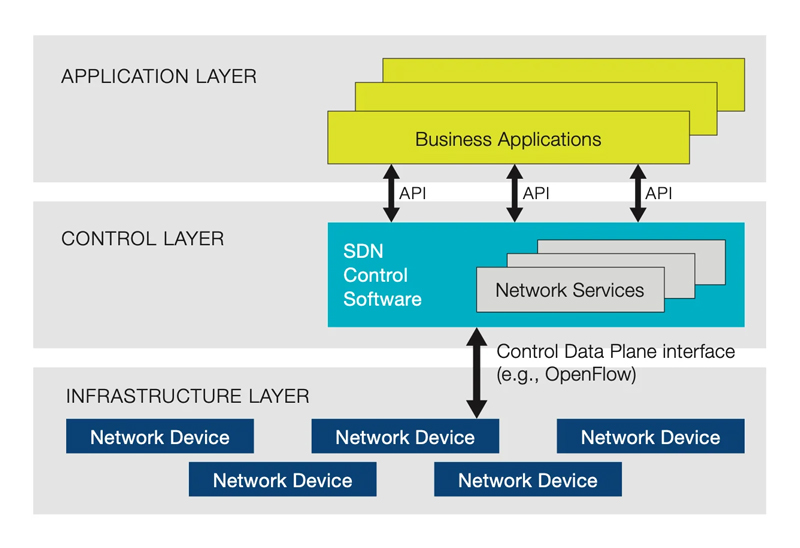
\includegraphics[
        width=0.9\textwidth,
        height=0.72\textheight,
        keepaspectratio
    ]{images/kien-truc-cua-software-defined-networking.jpg}

    \vspace{0.1cm}
    {\scriptsize\textit{Hình 2.1: Ba lớp chức năng trong kiến trúc Software-Defined Networking}}
\end{frame}

% --- SLIDE 2.3: SD-WAN ---
\begin{frame}{2.3 Software-Defined WAN (SD-WAN)}
    \begin{columns}[T]
        \column{0.48\textwidth}
        \textbf{Hai lớp mạng chính:}
        \begin{itemize}
            \item \textbf{Underlay:} hạ tầng truyền dẫn sẵn có như Internet hoặc MPLS.
            \item \textbf{Overlay:} mạng logic hình thành giữa các WAN Edge.
            \item Tunnel bảo mật vận chuyển dữ liệu giữa các site.
        \end{itemize}

        \column{0.48\textwidth}
        \textbf{Các vai trò điều khiển:}
        \begin{itemize}
            \item Quản lý tập trung và cung cấp thông tin vận hành.
            \item Điều phối việc tham gia overlay của thiết bị biên.
            \item Phân phối thông tin định tuyến và chính sách giữa các site.
        \end{itemize}
    \end{columns}
    \vspace{0.15cm}
    \begin{block}{Đặc trưng kiến trúc}
        Lớp overlay độc lập tương đối với hạ tầng truyền dẫn, nhờ đó có thể sử dụng nhiều loại đường WAN trong cùng một mô hình.
    \end{block}
\end{frame}

% --- SLIDE 2.4: So sánh vai trò ---
\begin{frame}{2.4 Vai trò của SDN và SD-WAN trong đề tài}
    \begin{table}
        \centering
        \small
        \renewcommand{\arraystretch}{1.35}
        \begin{tabular}{|p{0.2\textwidth}|p{0.35\textwidth}|p{0.35\textwidth}|}
            \hline
            \rowcolor{primaryDark!15}
            \textbf{Tiêu chí} & \textbf{SDN} & \textbf{SD-WAN} \\
            \hline
            Phạm vi & Mạng nội bộ trong Campus & Kết nối WAN giữa các cơ sở \\
            \hline
            Đối tượng & Switch và luồng dữ liệu nội bộ & WAN Edge, tunnel và route overlay \\
            \hline
            Trọng tâm & Điều khiển tập trung, chính sách luồng & Điều phối kết nối đa đường truyền \\
            \hline
            Giao thức tiêu biểu & OpenFlow & OMP, IPsec \\
            \hline
            Vai trò chung & \multicolumn{2}{c|}{Tách logic điều khiển khỏi hạ tầng chuyển tiếp} \\
            \hline
        \end{tabular}
    \end{table}
\end{frame}

% --- SLIDE 2.5: Nền tảng giao thức ---
\begin{frame}{2.5 Các giao thức và cơ chế nền tảng}
    \begin{columns}[T]
        \column{0.48\textwidth}
        \textbf{Trong Campus:}
        \begin{itemize}
            \item \textbf{VLAN/802.1Q:} phân tách miền quảng bá.
            \item \textbf{OSPF:} trao đổi thông tin định tuyến nội bộ.
            \item \textbf{VRRP:} cung cấp gateway logic dự phòng.
            \item \textbf{DHCP:} cấp phát tham số mạng cho đầu cuối.
        \end{itemize}

        \column{0.48\textwidth}
        \textbf{Trong SDN và SD-WAN:}
        \begin{itemize}
            \item \textbf{OpenFlow:} quản lý bảng flow trên switch.
            \item \textbf{OMP:} trao đổi route và thông tin overlay.
            \item \textbf{IPsec:} bảo vệ dữ liệu qua đường WAN.
            \item \textbf{ACL/Firewall:} kiểm soát truy cập giữa các vùng.
        \end{itemize}
    \end{columns}
\end{frame}

% =========================================================================
% CHAPTER 3: MÔ HÌNH NGHIÊN CỨU VÀ THIẾT KẾ ĐỀ XUẤT
% =========================================================================

\section{Mô hình nghiên cứu và Thiết kế đề xuất}

% --- SLIDE 3.1: Yêu cầu thiết kế ---
\begin{frame}{3.1 Yêu cầu đối với mô hình đề xuất}
    \begin{columns}[T]
        \column{0.48\textwidth}
        \textbf{Yêu cầu chức năng:}
        \begin{itemize}
            \item Kết nối người dùng và dịch vụ theo từng khu vực chức năng.
            \item Phân tách lưu lượng giữa các khoa, phòng ban và vùng máy chủ.
            \item Kết nối Campus chính với các cơ sở phụ.
            \item Hỗ trợ quản lý tập trung tại LAN và WAN.
        \end{itemize}

        \column{0.48\textwidth}
        \textbf{Yêu cầu kiến trúc:}
        \begin{itemize}
            \item Phân tầng rõ ràng, hạn chế phụ thuộc giữa các khối.
            \item Có đường truyền và gateway dự phòng ở vị trí quan trọng.
            \item Tách vùng người dùng, quản trị, máy chủ và DMZ.
            \item Cho phép biểu diễn đầy đủ trên môi trường mô phỏng.
        \end{itemize}
    \end{columns}
\end{frame}

% --- SLIDE 3.2: Kiến trúc tổng thể ---
\begin{frame}{3.2 Kiến trúc tổng thể đề xuất}
    \begin{columns}[T]
        \column{0.31\textwidth}
        \begin{block}{Campus chính}
            \centering
            Core--Distribution--Access\\
            SDN Controller\\
            Server Farm và DMZ
        \end{block}

        \column{0.31\textwidth}
        \begin{block}{Kết nối liên cơ sở}
            \centering
            WAN Edge\\
            Internet và MPLS\\
            SD-WAN Overlay
        \end{block}

        \column{0.31\textwidth}
        \begin{block}{Các cơ sở phụ}
            \centering
            Site 200 -- Cần Thơ\\
            Site 300 -- Đà Nẵng\\
            Site 400 -- Nha Trang
        \end{block}
    \end{columns}
    \vspace{0.2cm}
    \begin{block}{Nguyên tắc tích hợp}
        SDN điều khiển miền chuyển mạch trong Campus; SD-WAN đảm nhiệm kết nối giữa các site. Hai miền gặp nhau tại lớp Core/WAN Edge.
    \end{block}
\end{frame}

% --- SLIDE 3.3: Mô hình Campus chính ---
\begin{frame}{3.3 Mô hình Campus chính}
    \begin{columns}[T]
        \column{0.48\textwidth}
        \textbf{Kiến trúc phân tầng:}
        \begin{itemize}
            \item \textbf{Core:} kết nối các vùng chính, định tuyến và cung cấp gateway.
            \item \textbf{Distribution:} tổng hợp các nhánh Access và áp dụng chính sách.
            \item \textbf{Access:} kết nối thiết bị người dùng theo VLAN.
        \end{itemize}

        \column{0.48\textwidth}
        \textbf{Vị trí của SDN:}
        \begin{itemize}
            \item Controller cung cấp lớp điều khiển logic tập trung.
            \item Các switch Distribution/Access đảm nhiệm chuyển tiếp dữ liệu.
            \item Kênh điều khiển được tách khỏi lưu lượng người dùng.
        \end{itemize}
    \end{columns}
    \vspace{0.15cm}
    \begin{block}{Các vùng dịch vụ}
        Server Farm cung cấp dịch vụ nội bộ; DMZ chứa dịch vụ cần công bố; Firewall kiểm soát lưu lượng giữa các vùng.
    \end{block}
\end{frame}

% --- SLIDE 3.4: Phân vùng logic ---
\begin{frame}{3.4 Phân vùng logic và quy hoạch địa chỉ}
    \begin{table}
        \centering
        \small
        \renewcommand{\arraystretch}{1.3}
        \begin{tabular}{|p{0.22\textwidth}|p{0.3\textwidth}|p{0.38\textwidth}|}
            \hline
            \rowcolor{primaryDark!15}
            \textbf{Nhóm mạng} & \textbf{Đối tượng} & \textbf{Nguyên tắc thiết kế} \\
            \hline
            Người dùng & Khoa, phòng ban, phòng học & Một VLAN/subnet riêng cho mỗi nhóm \\
            \hline
            Dịch vụ nội bộ & DHCP, Syslog và dịch vụ dùng chung & Đặt trong Server Farm, địa chỉ ổn định \\
            \hline
            Dịch vụ công bố & Web, Mail & Tách riêng trong DMZ và đi qua Firewall \\
            \hline
            Quản trị & Controller và giao diện quản lý & Tách khỏi lưu lượng người dùng \\
            \hline
            Liên kết WAN & Các đường point-to-point & Dùng dải riêng cho underlay và định danh site \\
            \hline
        \end{tabular}
    \end{table}
\end{frame}

% --- SLIDE 3.5: Mô hình liên kết đa cơ sở ---
\begin{frame}{3.5 Mô hình kết nối đa cơ sở}
    \begin{columns}[T]
        \column{0.48\textwidth}
        \textbf{Underlay:}
        \begin{itemize}
            \item Internet và MPLS cung cấp khả năng truyền dẫn vật lý.
            \item Mỗi site kết nối vào WAN thông qua thiết bị biên.
            \item Định tuyến underlay bảo đảm khả năng tiếp cận giữa các WAN Edge.
        \end{itemize}

        \column{0.48\textwidth}
        \textbf{Overlay:}
        \begin{itemize}
            \item Các site trao đổi route logic thông qua lớp điều khiển SD-WAN.
            \item Dữ liệu liên cơ sở được vận chuyển qua tunnel bảo mật.
            \item Chính sách WAN được quản lý theo site và loại lưu lượng.
        \end{itemize}
    \end{columns}
    \vspace{0.15cm}
    \begin{block}{Phạm vi của mô hình}
        Campus chính và ba cơ sở phụ được biểu diễn trong cùng một topology để nghiên cứu quan hệ giữa mạng nội bộ và mạng WAN.
    \end{block}
\end{frame}

% =========================================================================
% CHAPTER 4: BÁO CÁO TIẾN ĐỘ NGHIÊN CỨU
% =========================================================================

\section{Báo cáo tiến độ nghiên cứu}

% Khung ảnh dùng cho các slide minh họa tiến độ. Khi có ảnh thật, thay lệnh
% \slideScreenshotPlaceholder bằng \includegraphics[...,keepaspectratio]{images/...}.
\newcommand{\slideScreenshotPlaceholder}[2]{%
    \begin{tcolorbox}[
        height=0.65\textheight,
        colback=lightGrayBg,
        colframe=accentTeal,
        boxrule=1pt,
        arc=0pt,
        valign=center
    ]
        \centering
        {\color{accentTeal}\fontsize{28}{30}\selectfont\faImage}\par
        \vspace{0.2cm}
        \textbf{#1}\par
        \vspace{0.12cm}
        {\scriptsize\color{black!60}\texttt{#2}}
    \end{tcolorbox}%
}

% --- SLIDE 4.1: Tổng quan tiến độ ---
\begin{frame}{4.1 Tổng quan tiến độ}
    \begin{table}
        \centering
        \scriptsize
        \setlength{\tabcolsep}{4pt}
        \renewcommand{\arraystretch}{1.28}
        \begin{tabular}{|p{0.33\textwidth}|p{0.18\textwidth}|p{0.42\textwidth}|}
            \hline
            \rowcolor{primaryDark!15}
            \textbf{Khối công việc} & \textbf{Trạng thái} & \textbf{Kết quả hiện tại} \\
            \hline
            Nghiên cứu Campus Network, SDN, SD-WAN & Hoàn thành & Đã hệ thống hóa khái niệm, thành phần và vai trò \\
            \hline
            Phân tích yêu cầu và phạm vi & Hoàn thành & Xác định mô hình đại học gồm Campus chính và ba cơ sở phụ \\
            \hline
            Thiết kế kiến trúc và phân vùng logic & Hoàn thành & Có mô hình phân tầng, VLAN/IP, Server Farm và DMZ \\
            \hline
            Xây dựng mô hình EVE-NG & Đang rà soát & Topology đã hình thành; tiếp tục đối chiếu kết nối và thiết bị \\
            \hline
            Tích hợp các khối SDN và SD-WAN & Đang thực hiện & Hoàn thiện quan hệ điều khiển và kết nối giữa các site \\
            \hline
            Kiểm thử và tổng hợp kết quả & Chưa thực hiện & Thực hiện sau khi mô hình được hoàn thiện \\
            \hline
        \end{tabular}
    \end{table}
\end{frame}

% --- SLIDE 4.2: Mẫu ảnh các Site Campus ---
\begin{frame}{4.2 Minh họa các Site Campus}
    \small
    \begin{columns}[T,onlytextwidth]
        \column{0.52\textwidth}
        \slideScreenshotPlaceholder{CHÈN ẢNH CHỤP SITE}{images/site-campus.png}

        \column{0.44\textwidth}
        \textbf{Cách thiết kế vùng Site:}
        \begin{itemize}
            \item Site 100 dùng mô hình \textbf{Core--Distribution--Access}; các site 200/300/400 được phân vùng theo khoa và VLAN nghiệp vụ.
            \item Mạng người dùng và mạng quản trị được tách thành các subnet riêng theo mã site.
            \item Firewall/WAN Edge tạo ranh giới giữa LAN Campus và mạng WAN.
            \item Prefix của từng site được trao đổi qua SD-WAN overlay.
        \end{itemize}
        \vspace{0.08cm}
        {\color{accentTeal}\textbf{Ảnh cần thể hiện:}} ranh giới site, switch, Firewall, vEdge và uplink về Service Provider.
    \end{columns}
\end{frame}

% --- SLIDE 4.3: Mẫu ảnh Service Provider ---
\begin{frame}{4.3 Service Provider và mạng Underlay}
    \small
    \begin{columns}[T,onlytextwidth]
        \column{0.52\textwidth}
        \slideScreenshotPlaceholder{CHÈN ẢNH INTERNET/MPLS}{images/service-provider-underlay.png}

        \column{0.44\textwidth}
        \textbf{Cách thiết kế vùng Underlay:}
        \begin{itemize}
            \item \textbf{Internet} dùng dải \texttt{203.0.113.0/24}; mỗi WAN Edge nối qua một liên kết transit \texttt{/30}.
            \item \textbf{MPLS} dùng các mạng \texttt{100.64.<site>.x/30} để tách kết nối theo site.
            \item Service Provider chỉ cung cấp IP reachability cho các WAN Edge.
            \item OMP và IPsec hình thành lớp overlay bên trên hai transport.
        \end{itemize}
        \vspace{0.08cm}
        {\color{accentTeal}\textbf{Ảnh cần thể hiện:}} hai cloud Internet/MPLS, các link tới vEdge và Site 900.
    \end{columns}
\end{frame}

% --- SLIDE 4.4: Mẫu ảnh SDN Controller ---
\begin{frame}{4.4 Vùng SDN Controller}
    \small
    \begin{columns}[T,onlytextwidth]
        \column{0.52\textwidth}
        \slideScreenshotPlaceholder{CHÈN ẢNH SDN CONTROLLER}{images/sdn-controller-zone.png}

        \column{0.44\textwidth}
        \textbf{Cách thiết kế vùng điều khiển:}
        \begin{itemize}
            \item Ryu Controller sử dụng \textbf{OpenFlow 1.3} để điều khiển lớp chuyển tiếp.
            \item Control Plane dùng VLAN 99 MANAGEMENT (dải \texttt{10.1.99.0/24}, controller \texttt{10.1.99.10}).
            \item Controller nối 1 cổng vào Server Farm, kênh điều khiển tới 6 switch OVS đi qua link uplink sẵn có.
            \item Lưu lượng điều khiển được tách khỏi Data Plane của người dùng.
        \end{itemize}
        \vspace{0.08cm}
        {\color{accentTeal}\textbf{Ảnh cần thể hiện:}} Controller, 6 switch OVS và kênh control plane trên VLAN quản trị.
    \end{columns}
\end{frame}

% --- SLIDE 4.5: Mẫu ảnh Server Farm ---
\begin{frame}{4.5 Vùng Server Farm}
    \small
    \begin{columns}[T,onlytextwidth]
        \column{0.52\textwidth}
        \slideScreenshotPlaceholder{CHÈN ẢNH SERVER FARM}{images/server-farm-zone.png}

        \column{0.44\textwidth}
        \textbf{Cách thiết kế vùng dịch vụ nội bộ:}
        \begin{itemize}
            \item Server Farm đặt trong \textbf{VLAN 90}, mạng \texttt{10.1.90.0/24}.
            \item DHCP Server \texttt{10.1.90.10} và Syslog Server \texttt{10.1.90.11} dùng địa chỉ tĩnh.
            \item SwitchServerFarm nối dự phòng tới Core-SW1/2 bằng trunk VLAN 90/99.
            \item Vùng dịch vụ được tách khỏi mạng người dùng và DMZ.
        \end{itemize}
        \vspace{0.08cm}
        {\color{accentTeal}\textbf{Ảnh cần thể hiện:}} switch tập trung, DHCP, Syslog và hai uplink Core.
    \end{columns}
\end{frame}

% --- SLIDE 4.6: Mẫu ảnh DMZ ---
\begin{frame}{4.6 Vùng DMZ}
    \small
    \begin{columns}[T,onlytextwidth]
        \column{0.52\textwidth}
        \slideScreenshotPlaceholder{CHÈN ẢNH DMZ}{images/dmz-zone.png}

        \column{0.44\textwidth}
        \textbf{Cách thiết kế vùng dịch vụ công bố:}
        \begin{itemize}
            \item DMZ dùng mạng \texttt{10.1.1.0/28}, tách khỏi Inside và Server Farm.
            \item Web Server \texttt{10.1.1.10} và Mail Server \texttt{10.1.1.11} nối qua SwitchDMZ.
            \item Cặp Firewall ASAv Active/Standby cung cấp gateway và kiểm soát luồng truy cập.
            \item Chỉ các dịch vụ cần công bố mới được phép đi qua chính sách Firewall.
        \end{itemize}
        \vspace{0.08cm}
        {\color{accentTeal}\textbf{Ảnh cần thể hiện:}} Firewall HA, SwitchDMZ, Web/Mail và ranh giới Inside--Outside.
    \end{columns}
\end{frame}

% --- SLIDE 4.7: Kết quả nghiên cứu đã hoàn thành ---
\begin{frame}{4.7 Nội dung đã hoàn thành}
    \begin{columns}[T]
        \column{0.48\textwidth}
        \textbf{Về lý thuyết:}
        \begin{itemize}
            \item Làm rõ mô hình Campus ba lớp và chức năng của từng lớp.
            \item Phân tích nguyên lý tách Control Plane/Data Plane trong SDN.
            \item Phân tích underlay, overlay và các vai trò điều khiển trong SD-WAN.
            \item Xác định vị trí tích hợp SDN và SD-WAN trong kiến trúc chung.
        \end{itemize}

        \column{0.48\textwidth}
        \textbf{Về thiết kế:}
        \begin{itemize}
            \item Xác định bốn site và miền điều khiển SD-WAN.
            \item Hoàn thiện nguyên tắc phân vùng VLAN và quy hoạch địa chỉ.
            \item Phân tách vùng người dùng, quản trị, Server Farm và DMZ.
            \item Xây dựng topology làm cơ sở cho giai đoạn mô phỏng.
        \end{itemize}
    \end{columns}
\end{frame}

% --- SLIDE 4.8: Công việc đang thực hiện ---
\begin{frame}{4.8 Công việc đang thực hiện}
    \begin{block}{Trọng tâm hiện tại}
        Hoàn thiện sự nhất quán giữa cơ sở lý thuyết, thiết kế logic và topology mô phỏng.
    \end{block}
    \vspace{0.15cm}
    \begin{enumerate}
        \item Rà soát vai trò và kết nối của các khối Core, Distribution, Access, Firewall và WAN Edge.
        \vspace{0.12cm}
        \item Đối chiếu VLAN, subnet và vùng dịch vụ với yêu cầu của từng site.
        \vspace{0.12cm}
        \item Hoàn thiện mô hình điều khiển tập trung cho các switch trong Campus chính.
        \vspace{0.12cm}
        \item Hoàn thiện quan hệ underlay/overlay giữa Campus chính và các cơ sở phụ.
        \vspace{0.12cm}
        \item Chuẩn bị các kịch bản kiểm tra kết nối cơ bản cho giai đoạn tiếp theo.
    \end{enumerate}
\end{frame}

% --- SLIDE 4.9: Phần việc tiếp theo trong phạm vi đề tài ---
\begin{frame}{4.9 Kế hoạch hoàn thành giai đoạn hiện tại}
    \begin{enumerate}
        \item \textbf{Hoàn thiện mô hình:} rà soát topology, địa chỉ và quan hệ giữa các thành phần.
        \vspace{0.15cm}
        \item \textbf{Kiểm tra chức năng cơ bản:} kết nối trong cùng VLAN, giữa các VLAN và giữa các site.
        \vspace{0.15cm}
        \item \textbf{Ghi nhận kết quả:} thu thập sơ đồ, bảng trạng thái và minh chứng từ mô phỏng.
        \vspace{0.15cm}
        \item \textbf{Hoàn thiện báo cáo:} đồng bộ phần lý thuyết, thiết kế và tiến độ thực hiện.
    \end{enumerate}
    \vspace{0.2cm}
    \begin{block}{Giới hạn của kế hoạch}
        Chỉ tập trung hoàn tất các hạng mục đã xác định trong đề tài, không mở rộng thêm công nghệ hoặc phạm vi mới.
    \end{block}
\end{frame}

% =========================================================================
% CHAPTER 5: KẾT LUẬN BÁO CÁO TIẾN ĐỘ
% =========================================================================

\section{Kết luận báo cáo tiến độ}

\begin{frame}{5.1 Kết luận tạm thời}
    \begin{enumerate}
        \item \textbf{Cơ sở lý thuyết:}
        \par Đã hệ thống hóa kiến trúc Campus phân cấp, nguyên lý SDN và mô hình kết nối SD-WAN.
        \vspace{0.18cm}
        \item \textbf{Mô hình đề xuất:}
        \par Đã xác định vai trò của SDN trong Campus, SD-WAN giữa các cơ sở và vị trí tích hợp của hai miền.
        \vspace{0.18cm}
        \item \textbf{Thiết kế logic:}
        \par Đã xây dựng phân tầng mạng, phân vùng chức năng và nguyên tắc quy hoạch địa chỉ cho mô hình đa site.
        \vspace{0.18cm}
        \item \textbf{Tiến độ hiện tại:}
        \par Topology mô phỏng đã hình thành; công việc đang tập trung vào rà soát tính nhất quán và chuẩn bị kiểm tra chức năng cơ bản.
    \end{enumerate}
\end{frame}


\end{document}
